\chapter{Fenómenos de transporte en semiconductores}



En este tema estudiarmemos los fenómenos de transporte en semiconductores, que son varios. Dedicaremos una sección a cada uno de ellos:

\begin{itemize}
	\item Arrastre.
	\item Difusión.
	\item Generación.
	\item Recombinación.
	\item Emisión termoiónica.
	\item Trasmisión túnel.
	\item Ionización por impacto.
\end{itemize} 
Además veremos \textit{ecuaciones básicas de trasnporte} y métodos de medida de parámetros como resistividad, movilidades, concentración, tiempos de vida, etc.


%%%%%%%%%%%%%%%%%%%%%%%%%%%%%%%%%%%%%%%%%%%%%%%%%%%%%%%%%%%%%%%%%%%%%%%
%%%%%%%%%%%%%%%%%%%%%%%%%%%%%%%%%%%%%%%%%%%%%%%%%%%%%%%%%%%%%%%%%%%%%%%
%%%%%%%%%%%%%%%%%%%%%%%%%%%%%%%%%%%%%%%%%%%%%%%%%%%%%%%%%%%%%%%%%%%%%%%
%%%%%%%%%%%%%%%%%%%%%%%%  TEMA 1 %%%%%%%%%%%%%%%%%%%%%%%%%%%%%%%%%%
%%%%%%%%%%%%%%%%%%%%%%%%%%%%%%%%%%%%%%%%%%%%%%%%%%%%%%%%%%%%%%%%%%%%%%%
%%%%%%%%%%%%%%%%%%%%%%%%%%%%%%%%%%%%%%%%%%%%%%%%%%%%%%%%%%%%%%%%%%%%%%%
%%%%%%%%%%%%%%%%%%%%%%%%%%%%%%%%%%%%%%%%%%%%%%%%%%%%%%%%%%%%%%%%%%%%%%%

\section{Arrastre}

\subsection{Introducción: modelo de arrastre y difusión}

El \textbf{modelo de arrastre-difusión} considera que las corrientes en el interior del semiconductor se debe exclusivamente a dos componentes: arrastre y difusión. 

\begin{itemize}
	\item \textbf{Arrastre:} movimiento de los portadores provocado por campos eléctricos externos e internos.
	\item \textbf{Difusión:} movimiento de portadores debido a gradientes de concentración debido a gradientes de concentracion. En la difusión los portadores se desplazarán de donde son mayoritarios a donde son minoritarios.
\end{itemize}
Así pues, según este modelo, las corrientes de portadores electrón $J_n$ y de portadores hueco $J_p$ serán iguales a la suma de las componentes de arrastre y difusión:

\begin{equation}
	J_n =  {J_n}|_{\text{arrastre}} + {J_n}|_{\text{difusión}} \tquad
	J_p =  {J_p}|_{\text{arrastre}} + {J_p}|_{\text{difusión}} 
\end{equation}
siendo la \textit{corriente total} la suma de ambas componentes: 

\begin{equation}
	J = J_n + J_p
\end{equation}

\subsection{Corriente de arrastre}

Si no aplicamos ninguna fuerza externa, el movimiento de los electrones a tempeartura no nula será un proceso aleatorio, en el que se sucederán colisiones con átomos de la red, impurezas, fonones, fotones... de tal manera que \textit{el movimiento efectivo es nulo}. Sin embargo los electrones si poseen velocidad, la cual podemos calcular, en virtud del \textit{teorema de equipartición}, tal que por cada grado de libertad del electrón le asignamos $kT/2$ de energía cinética. Como en el modelo de semiconductores, los huecos y electrones en las bandas de valencia y conducción son partículas libres (con masa efectiva diferente a $m_e$, pero partículas libres a fin de cuentas), podemos aplicarles el teorema de equipartición, tal que:

\begin{equation}
	\frac{1}{2} m^* v_{th}^2 = \frac{3}{2} kT
\end{equation}
siendo $v_{th}$ la \textit{velocidad media de cada partícula}. Cuando aplicamos un campo eléctrico $\Ecal$, todos los portadores experimentarán una fuerza $q\Ecal$, que lo acelera entre las sucesivas colisiones. Esta fuerza aplicada sobre el semiconductor provocará un desplazamiento neto de electrones en la dirección opuesta al campo y de huecos en la dirección del campo. Definimos entonces dos parámetros fundamentales: \textbf{camino medio recorrido} $\lambda$, que es la distancia media entre dos colisiones $(\sim 10^{-5} \cm$) y el \textbf{tiempo medio recorrido} $\tau$, que es el tiempo medio entre dos colisiones ($\sim 10^{-12} s$). 

Supongamos entonces que los portadores se mueven a una velocidad constante $v_a$ (que lógicamente dependerá de la temperatura, de la fuerza del campo...). Como hemos visto en el tema anterior, un hueco es una partícula virtual igual al electrón en todo exceptuando que tiene carga positiva. Si consideramos que el electrón se mueve a una velocidad constante $v_a$, el hueco también lo hará. En ese caso la densidad de corriente no es más que:

\begin{equation}
	J_n|_{\text{arrastre}} = -qnv_a \tquad 	J_p|_{\text{arrastre}} = qpv_a
\end{equation}
siendo $q$ la carga. Tal y como hemos dicho, la velocidad $v_a$ no es una constante del material, sino que depende de variables tales como la temperatura, el grado de impurezas o de la intensidad del campo. De manera experimental se sabe, que bajo campos no muy intensos, la velocidad tiene una dependencia lineal con el campo eléctrico, véase \cref{Fig:02-01}. 

\begin{figure}[h!] \centering
	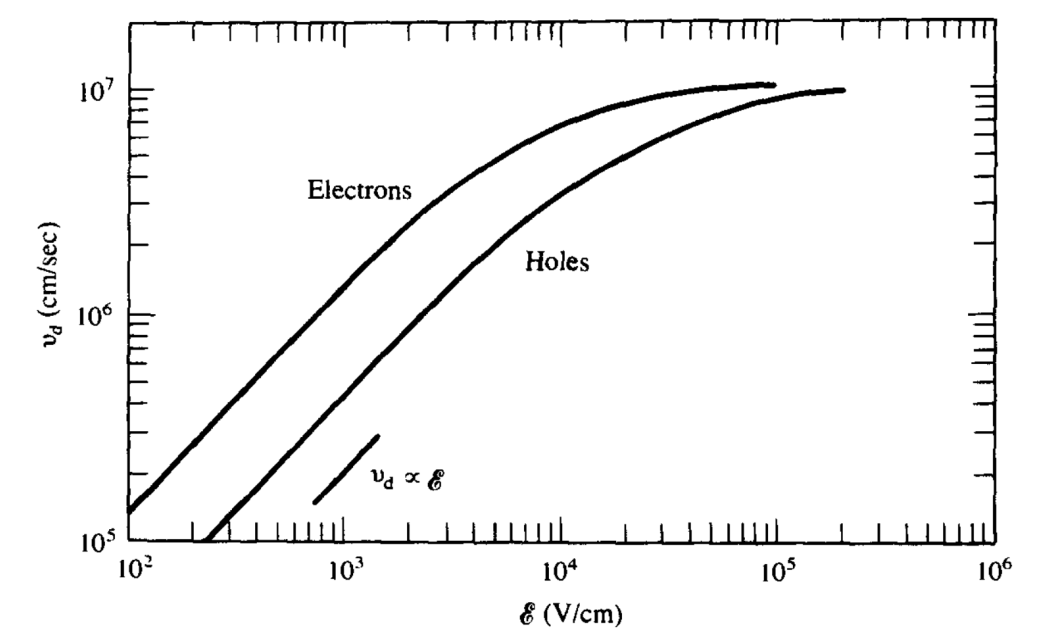
\includegraphics[width=0.9\linewidth]{Cuerpo/Ch_02/02_Movilidad_E.png}
	\caption{Movilidad frente a campo eléctrico. Véase que en la región de campo débil sigue una ecuación lineal, hasta que en campo fuerte se hace constante.}
	\label{Fig:02-01}
\end{figure}
La constante que relaciona la velocidad y el campo eléctrico se llama \textbf{movilidad} y se denota por $\mu$. Así pues, $\mu_n$ es la movilidad del electrón y $\mu_p$ la del hueco, y verifican:

\begin{equation}
	v_n = - \mu_n \Ecal \tquad v_p = \mu_p \Ecal
\end{equation}
midiéndose en $\cm^2/$Vs. Entonces la corriente de arrastre es:

\begin{equation}
	J_{\text{arrastre}} = qn\mu_n \Ecal + qp\mu_p \Ecal = q(n\mu_n+p\mu_p)\Ecal
\end{equation}
\subsection{Dispersión: efectos en la movilidad}

La movilidad, a su vez, depende del grado de dispersión. Si la dispersión es muy baja la movilidad es muy alta: los electrones chocan poco y se pueden acelerar mucho. Como fuentes de dispersión tenemos: \textit{fonones, átomos dopantes ionizados, aleaciones, imperfecciones en la red, defectos en las interfaces...} Los fenómenos que más influencia tienen son:

\begin{itemize}
	\item Dispersión por choques entre portadores (poca influcencia).
	\item Dipsersión por la red cristalina (choques de los portadores con los átomos de la red, que dominan a alta temperatura).
	\item Dispersión por dopantes ionizadas (choques con impurezas donadores o aceptadoras, que dominan a baja temperatura).
\end{itemize}
Consecuentemente tenemos dos efectos principales, el efecto debido a las impurezas y el efecto debido a los fonones. La probabildiad de colisión por unidad de tiempo global es la suma de las probabilidades parciales de cada tipo de colisión, según la \textit{regla matthiessen}:

\begin{equation}
	\frac{1}{\tau_c} = \frac{1}{\tau_c|_{\text{fonones}}}+\frac{1}{\tau_c|_{\text{impurezas}}}
\end{equation}
Y en términos de la movilidad:

\begin{equation}
	\frac{1}{\mu}=\frac{1}{\mu_F}+\frac{1}{\mu_I}
\end{equation}
lógicamente esto es \textit{generalizable}, pudiendo incluir los mecanismos de dispersión.

\begin{figure}[h!] \centering
	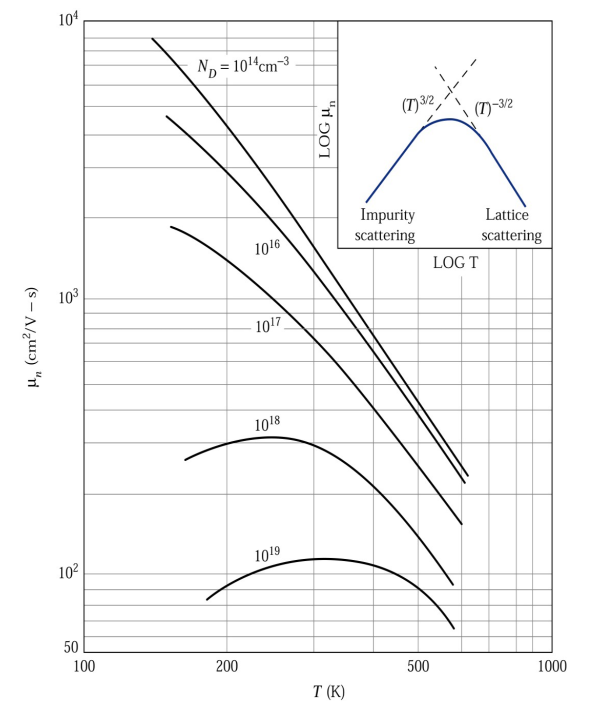
\includegraphics[width=0.6\linewidth]{Cuerpo/Ch_02/02_Movilidad.png}
	\caption{Movilidad en función de $T$.}
	\label{Fig:02-02}
\end{figure}

\subsubsection{Dispersión por impurezas}

\subsubsection{Dispersión por fonones}


\subsection{Resistividad y movilidad}

La \textbf{resistividad} ($\rho$) se define como la constante de proporcionalidad entr el campo eléctrico aplicado y la corriente total de carga por unidad de área que fluye en el mismo (suponiendo un material homogéneo). Al inverso de la resistividad lo llamamos \textbf{conductividad} ($\sigma$) tal que

\begin{equation}
	\sigma \equiv \frac{1}{\rho}
\end{equation}
Como sabemos $\Jn_{\text{arrastre}}=q(\mu_nn+\mu_pp)\Encal$. Entonces podemos relacionar la resistividad/conductividad de un material con la movilidad, tal que

\begin{equation}
	\rho = \frac{1}{q(\mu_n n + \mu_p p)}
\end{equation}

\subsection{Curvatura de bandas}

El campo eléctrico se puede estudiar y entender como el gradiente de una función llamada \textit{potencial escalar} que representa la energía por unidad de carga. Así pues, la acción de un campo eléctrico en un semiconductor hace que aparezca una diferencia de energía entre los diferentes puntos del semiconductor, haciendo que las bandas a lo largo del semiconductor no tengan la misma energía, tal y como podemos ver en .

\begin{figure}[h!] \centering
	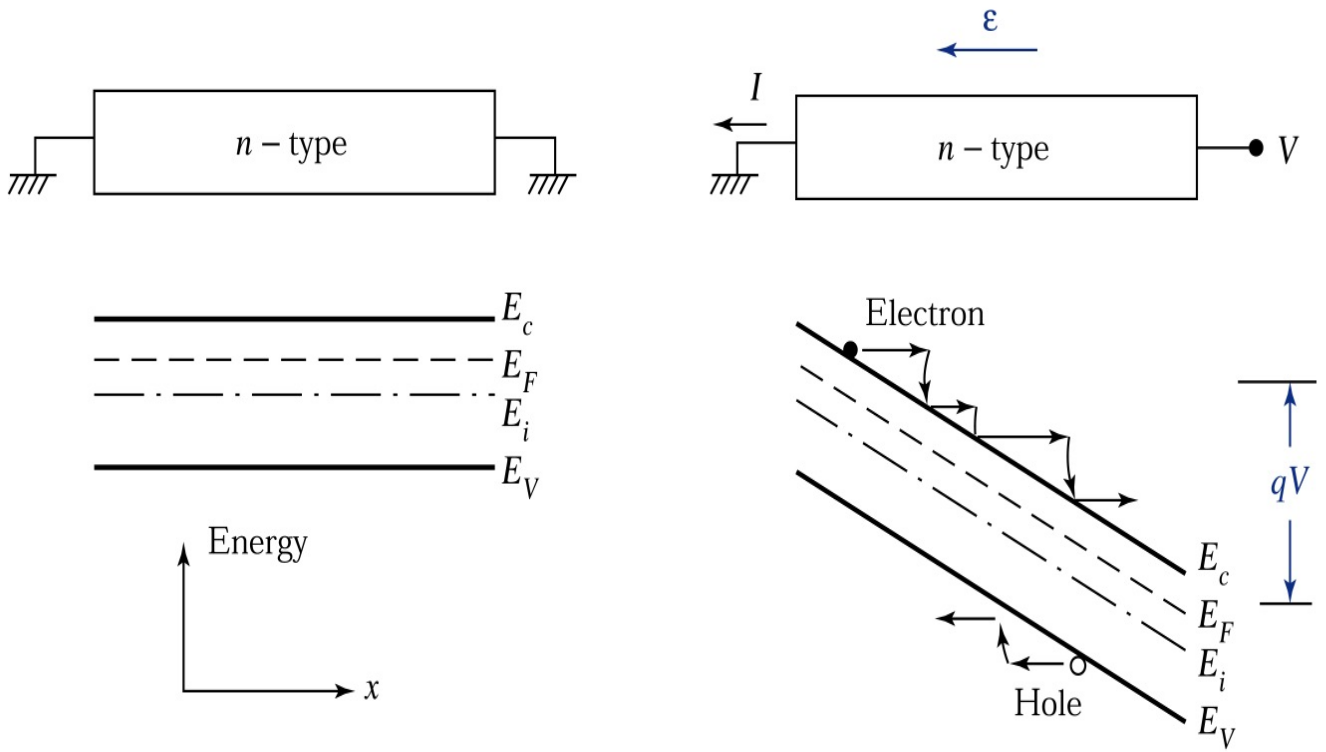
\includegraphics[width=0.8\linewidth]{Cuerpo/Ch_02/02_Campo_E.png}
	\caption{Efecto de un campo eléctrico externo en las bandas.}
	\label{Fig:02-03}
\end{figure}

Si $\psi$ es el \textit{potencial escalar eletroestático}, tenemos que:

\begin{equation}
	\Encal = \frac{1}{q} \derivadas{E_c}{x}= \frac{1}{q} \derivadas{E_i}{x}=- \derivadas{\psi}{x}
\end{equation}


%%%%%%%%%%%%%%%%%%%%%%%%%%%%%%%%%%%%%%%%%%%%%%%%%%%%%%%%%%%%%%%%%%%%%%%
%%%%%%%%%%%%%%%%%%%%%%%%%%%%%%%%%%%%%%%%%%%%%%%%%%%%%%%%%%%%%%%%%%%%%%%
%%%%%%%%%%%%%%%%%%%%%%%%%%%%%%%%%%%%%%%%%%%%%%%%%%%%%%%%%%%%%%%%%%%%%%%
%%%%%%%%%%%%%%%%%%%%%%%%  TEMA 2 %%%%%%%%%%%%%%%%%%%%%%%%%%%%%%%%%%
%%%%%%%%%%%%%%%%%%%%%%%%%%%%%%%%%%%%%%%%%%%%%%%%%%%%%%%%%%%%%%%%%%%%%%%
%%%%%%%%%%%%%%%%%%%%%%%%%%%%%%%%%%%%%%%%%%%%%%%%%%%%%%%%%%%%%%%%%%%%%%%
%%%%%%%%%%%%%%%%%%%%%%%%%%%%%%%%%%%%%%%%%%%%%%%%%%%%%%%%%%%%%%%%%%%%%%%


\section{Difusión}

La difusión es un proceso por el cual las partículas tienden a dispersarse o redistribuirse como restultado de su alta concentración en ciertas zonas del sólido o bajas concentraciones en otra zona a temperatura no nula. En este caso las partículas que sufren difusión son electrones y huecos, que harán aparecer corrientes de difusión.

\subsection{Corrientes de difusión}

La \textbf{ley de Flick} nos dice que las corrientes de difusión son directamente proporcionales a los gradientes de concetración de partículas, esto es:

\begin{equation}
	J_p|_{\text{difusión}} = -qD_p\nabla p \tquad
	J_n|_{\text{difusión}} =  qD_n\nabla n
\end{equation}
siendo $D_p$ y $D_n$ las llamadas \textit{constantes de difusión}, que dependen básicamente de dos términos: la velocidad media de nuestras partículas $v_{th}$ y el camino medio recorrido $\lambda$, tal que:

\begin{equation}
	D_n = v_{th} \lambda_{n} \qquad D_p = v_{th} \lambda_{p}
\end{equation}
En palabras: la capacidad de una partícula para difundirse depende tanto de qué tan rápido se mueve como de la distancia que recorre antes de cambiar de dirección. Para verlo mejor: imagina que una partícula se mueve en un entorno donde, cada cierto tiempo, choca y cambia de rumbo. Cuanto mayor sea su velocidad y mayor sea la distancia que recorre entre choques, más lejos llegará en promedio en un mismo intervalo de tiempo. Así, el producto de estos dos factores (velocidad y distancia entre colisiones) te da una medida de la eficacia con la que la partícula se dispersa en el medio. Esta difusión generará entonces la corriente de difusión de portadores tipo $n$ y tipo $p$.

\begin{equation}
	J_n |_{\text{difusion}} = qD_n \derivadas{n}{x} \qquad 	
	J_p |_{\text{difusion}} = -qD_p \derivadas{p}{x}
\end{equation}

\subsection{Relaciones de Einstein}

Las relación de Einstein para electrones nos permite relacionar el coeficiente de difusión y la movilidad para cada uno de los portadores con su carga y la temperatura del medio. La deducción de estas es trivial, ya que es consdierar que el semiconductor está en equlibrio y no degenerado

\begin{equation}
	J_n |_{\text{difusion}} +J_n |_{\text{arrastre}} = q\mu_n n \Encal + qD_n\derivadas{n}{x} = 0
\end{equation}
tal que 

\begin{equation}
	n=n_i e^{(E_F-E_i)/kT} \Rightarrow \derivadas{n}{x} = - \frac{n_i}{kT} e^{(E_F-E_i)/kT} \derivadas{E_i}{x} = - \frac{n}{kT} \derivadas{E_i}{x} = - \frac{q}{kT} \Encal
\end{equation}
de lo cual se deduce 

\begin{equation}
	J_n = (qn\Encal) \mu_n - qD_n \frac{q}{kT} n \Encal = 0
\end{equation}
resolviendo obtenemos la \textbf{relación de Einstein para los electrones}

\begin{equation}
	\frac{D_n}{\mu_n} = \frac{kT}{q}
\end{equation}
válida para semiconductores no degenerados tanto en equlibrio como fuera de él.



%%%%%%%%%%%%%%%%%%%%%%%%%%%%%%%%%%%%%%%%%%%%%%%%%%%%%%%%%%%%%%%%%%%%%%%
%%%%%%%%%%%%%%%%%%%%%%%%%%%%%%%%%%%%%%%%%%%%%%%%%%%%%%%%%%%%%%%%%%%%%%%
%%%%%%%%%%%%%%%%%%%%%%%%%%%%%%%%%%%%%%%%%%%%%%%%%%%%%%%%%%%%%%%%%%%%%%%
%%%%%%%%%%%%%%%%%%%%%%%%  TEMA 3 %%%%%%%%%%%%%%%%%%%%%%%%%%%%%%%%%%
%%%%%%%%%%%%%%%%%%%%%%%%%%%%%%%%%%%%%%%%%%%%%%%%%%%%%%%%%%%%%%%%%%%%%%%
%%%%%%%%%%%%%%%%%%%%%%%%%%%%%%%%%%%%%%%%%%%%%%%%%%%%%%%%%%%%%%%%%%%%%%%
%%%%%%%%%%%%%%%%%%%%%%%%%%%%%%%%%%%%%%%%%%%%%%%%%%%%%%%%%%%%%%%%%%%%%%%

\section{Procesos de generación y recombinación}

Cuando un semiconductor es perturbado de su estado de equilibrio, el semiconductor responde modificando el número de portadores que hay en el mismo. La recombinación-generación (denotada por RG o R-G) es el mecanismo con el que describimos el proceso por el cual un exceso o deficiencia de portadores se estabiliza (si la perturbación se mantiene en el tiempo) o es eliminada (si la perturbación es temporal). Dado que durante la perturbación el sistema está bajo condiciones de no equilibrio, muchas de los fenómenos que aparecen en el semiconductor no puedan ser descritos a través de los procesos RG. 

\subsection{Introducción}

En un semiconductor definimos como \textbf{recombinación} al proceso por el cual electrones y huecos son aniquilados/destruidos, mientras que la \textbf{generación} es el proceso por el cual electrones y huecos son creados. Esta descripción así hecha es muy general, y por tanto varios tipos de procesos podrían incluirse en lo que llamamos RG. Generalmente se usan las gráficas de banda energética para describir visualmente cuales son los posibles procesos RG, aunque sea solo para entender su naturaleza. También se suele describir que papel tiene la energía y que tipo de energía se emite/absorbe en estos procesos. 

\subsubsection{Procesos de recombinación}

Existen varios tipos de procesos de recombinación:

\begin{itemize}
	\item \textbf{Recombinación directa}. Es el tipo más simple de recombinación. En este hay una aniquilación directa entre un hueco en la banda de valencia y un electrón en la banda de conducción, en el que el electrón <<cae>> a la banda de valencia. Es un proceso típicamente radiativo, en el que el exceso de energía se convierte en un fotón de luz. 
	
	\item \textbf{Recombinación de centro RG}. Recordemos que las impurezas generan niveles energéticos en la región del gap de energía. Los defectos cristalinos, particularmente las impurezas atómicas, pueden generar niveles energéticos en medio del gap. En este proceso de recombinación, los llamados centros RG con energía $E_T$ actúan como intermediarios. Existen varios tipos de recombinaciones de centro RG. En la primera de ellas tanto el electrón en la BC y el hueco en la BV se ven atraídos al mismo centro RG, aníquilándose. Otra posibilidad es que un portador salte a la banda contrario usando el centro RG como mediador. A este proceso se le llama \textit{recombinación termal}, ya que no es un proceso radiativo (no emite fotones), emitiendo calor, o, en su defecto, fonones. También existen recombinaciones de centro RG usando como centros RG los niveles energéticos de los dadores y aceptores (que recordemos están muy cerca de los niveles energéticos de las bandas), aunque no son tan comunes. Estos procesos son radiativos, pero poco probables, y se denominan \textit{recombinación a través de niveles profundos}. No son tan probables porque, a temperaturas ambientes, la probabilidad de que vuelvan a excitarse al nivel de la banda de conducción es altamente probable.
	
	\item \textbf{Recombinación Auger} En el proceso Auger lo que ocurre es que una recombinación directa/de centro RG ocurre simultáneamente con la colisión de dos portadores. Consecuentemente, estos portadores altamente energéticos se <<termalizan>>  (pierden energía en pasos pequeños mediante pequeñas colisiones con la red cristalina). La dispersión posterior del electrón que se lleva toda la energía sucede a través de diferentes pasos, como una <<escalera>>, lo cual sucede  porque la relajación del portador energético no es un proceso instantáneo, sino que sucede en varias etapas debido a la dispersión con fonones. Los fonones (vibraciones cuánticas de la red cristalina) tienen energías discretas, lo que significa que el portador pierde energía en múltiplos de estas energías fonónicas. En semiconductores típicos, los fonones ópticos tienen energías del orden de decenas de meV, por lo que un electrón altamente excitado no puede perder toda su energía de golpe, sino que la va cediendo en `saltos'' discretos al emitir fonones ópticos uno tras otro.
	
	\item \textbf{Recombinación superficial}: 
\end{itemize}

\begin{Anotacion}
	\textcolor{red}{Importante colocar las imagenes}
\end{Anotacion}

\subsubsection{Procesos de generación}

Existen varios tipos de generación, uno por cada uno de los procesos de recombinación. Así pues, existe generación directa, la cual necesita energía térmica o electromagnética (a través de fotones); generación por centros RG (energía térmica), y en último lugar la generación a través de impactos ionizantes (proceso inverso a la recombinación Auger). En estos último, el par de portadores se genera como consecuencia del impacto de un portador con un átomo cristalino. La generación de portadores a través de impacto ionizante ocurre recurrentemente cuando hay regiones con un campo eléctrico $\Ecal$ muy alto, y es el responsable de los fenómenos de avalancha de las uniones $pn$.

\subsection{Consideraciones acerca los procesos RG}

Los procesos de recombinación y generación ocurren permanentemente, incluso en el equilibrio termodinámico, siendo el principal problema de los procesos RG el cálculo del ratio de producción de los diferentes procesos. Típicamente, uno solo necesita centrarse en el proceso principal (el que mayor ratio de producción tiene). En los semiconductores dopados no degenerados a una temperatura ambiente, uno esperea que los procesos dominantes sean procesos directos o de centro RG. 

Conociendo la forma de las bandas de energía (más concretamente, cual es el valor de $k$ para el cual la energía de la banda de conducción es mínima) podremos dilucidad cual de los procesos es dominante: o de tipo directo o de centro RG. ¿Cómo? Pues es bien sencillo: los fotones, al ser partículas sin masa, son capaces de llevar muy poco momento, y por tanto las transiciones son casi verticales, es decir, solo son capaces de describir los semiconductores de tipo directo (mínimo BC y máximo de BV en $k=0$). Por otro lado, los fonones pueden trasmitir momentos y energía mucho mas grandes, por lo que son capaces de describir tanto los procesos en los semiconductores directos e indirectos, aunque en el caso de los directos no es un proceso dominante. Los procesos térmicos están relacionados con la recombinación de centro RG y los procesos fotónicos con la recombinación directa, y por tanto podemos diferenciar cuando uno y otro son dominantes. 

\subsection{Recombinación directa en semiconductores de gap directo}

Definimos como $G$ ($R$) el número de pares electrones (huecos) generados $/\mathrm{cm}^3\mathrm{s}$. Estas tasas de recombinación y generación dependen en general del número de huecos y electrones que haya en el medio, por lo que en general:

\begin{equation}
	R = \beta np \tquad G = \alpha np
\end{equation} 
Para un conductor en equilibrio termodinámico $G_{th}=R_{th}$ (siendo estas las tasas de generación/combinación en el equilibrio), manteniéndose $n$ y $p$ constantes. En el equilibrio  $R = G = \beta n_{n0}p_{n0}$.

\begin{figure}[h!] \centering 
	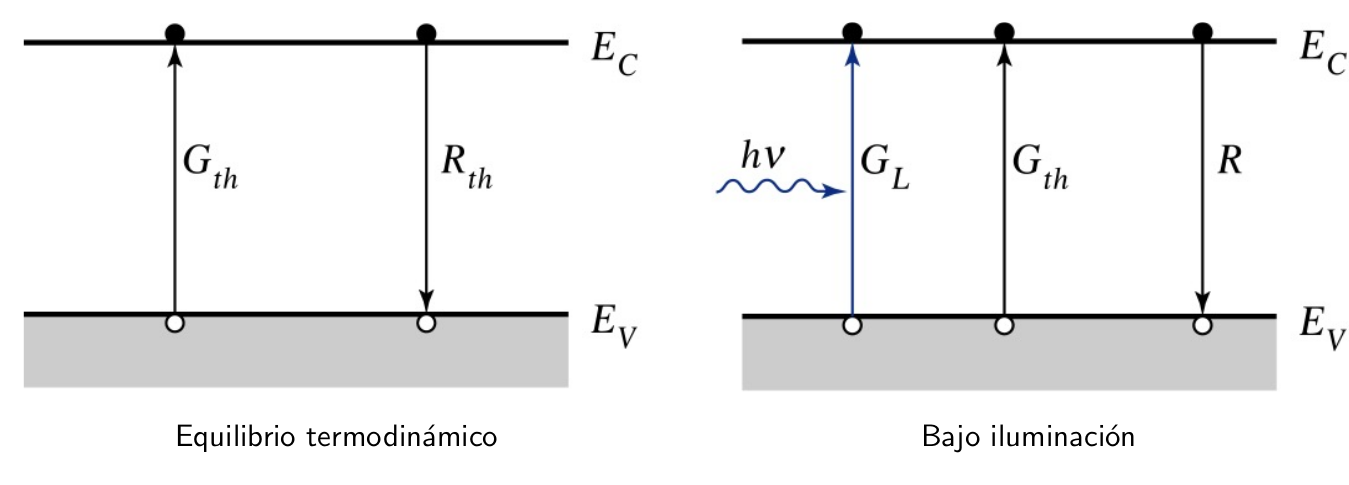
\includegraphics[width=0.9\linewidth]{Cuerpo/Ch_02/02_Luz.png}
	\caption{Procesos de generación y recombinación en equilibrio y sin luz.}
\end{figure}
Ahora bien, cuando iluminamos uno de estos semiconductores aumenta su generación en un término $G_L$, tal que ahora $G=G_L+G_{th}$. Consecuentemente tenemos que se incrementa en un número determinado el número de portadores en el semiconductor $\Delta n$ y $\Delta p$ ($\Delta n = \Delta p$, neutralidad de carga). Así pues tenemos que la tasa:


\begin{equation}
	\derivadas{p_n}{t} = G-R=G_L + G_{th} - R \tquad R = \beta n_n p_n = \beta (n_{n0}+\Delta n) (p_{n0}+\Delta p)
\end{equation}
Una vez llegamos al estado estacionario, podemos obtener entonces lo que llamamos el  \textit{ratio de recombinación} $U=R-G_{th}$, esto es:

\begin{equation}
	U = R-G_{th} = \beta (n_{n0}+p_{n0}+\Delta p)\Delta p
\end{equation}
Cuando tenemos $p_{n0}<<n_{n0}$ (bajo nivel de inyección tipo N), tenemos que:

\begin{equation}
	U = \beta n_{n0}\Delta p = \frac{p_n - p_{n0}}{\frac{1}{\beta n_{n0}}} =  \frac{p_n - p_{n0}}{\tau_p}
\end{equation}

\subsection{Recombinación indirecta en semiconductores de gap indirecto: procesos RG.}

\subsubsection{Definición de términos}

La estadística RG es el nombre que se le da a la caracterización matemática de los procesos de recombinación y generación. Dado que los procesos RG cambian las concentraciones de los portadores con el tiempo, la <<caracterización matemática>> de estos procesos no es más que la definición de las relaciones entre $\partial n / \partial t$ y $\partial p / \partial t$. Recordemos que los procesos RG lo que hacen es insertar una banda energética $E_T$ en la posición central del gap de bandas. Así pues definimos: 

\begin{itemize}
	\item Variación de $n$ debida a procesos RG: $\eval{\parciales{n}{t}}_{R_G}$.
	\item Variación de $p$ debida a procesos RG: $\eval{\parciales{p}{t}}_{R_G}$.
	\item Número de centros RG llenos de electrones por $\mathrm{cm}^3$: $n_T$.
	\item Número de centros RG llenos de huecos por $\mathrm{cm}^3$ $p_T$
	\item Número total de centros RG por $\mathrm{cm}^3$: $N_T$
\end{itemize}
Es importante que quede muy claro que $\partial n / \partial t |_{RG}$ y $\partial p / \partial t|_{RG} $ son tasas netas, teniendo en cuenta tanto los procesos de recombinación como los procesos de generación. Cuando $\partial n / \partial t|_{RG}$ es negativo, la tasa de neta de electrones es negativa $R>G$; y si es postiva, la tasa de electrones es positiva $G>R$. La desingación de $|_{RG}$ no denota otra cosa que <<tasa de cambio producida por los procesos RG>>. Esto es importante, ya que pueden ocurrir otros procesos además de estos. 

\subsubsection{Obtención de las tasas de producción} 

Existiendo 4 tipos de transiciones RG, que son:

\begin{itemize}
	\item \textbf{Captura de un electrón en un centro RG}. Se define $c_n$ como el \textit{coeficiente de captura de electrones} $(\text{cm}^3/s)$ con signo positivo. 
	\item \textbf{Emisión de un electrón por un centro RG}.Se define $e_n$ como el \textit{coeficiente de emisión de electrones} $(\text{cm}^3/s)$ con signo positivo. 
	\item \textbf{Captura de un hueco en un centro de RG} (o un electrón de un RG cae a BV). Se define $c_p$ como el \textit{coeficiente de captura de huecos} $(\text{cm}^3/s)$ con signo positivo. 
	\item \textbf{Emisión de un hueco por un centro de RG} (o un electrón de BV cae a RG). Se define $e_p$ como el \textit{coeficiente de emisión de electrones} $(\text{cm}^3/s)$ con signo positivo.  
\end{itemize}
Una vez entendemos esto, es claro que las ecuaciones que rigen los procesos RG son (no pueden ser de otra forma)

\begin{equation}
	r_N = \eval{\parciales{n}{t}}_{R_G} = e_n n_T - c_n n p_T \tquad r_P = 	\eval{\parciales{p}{t}}_{R_G} = e_pp_T - c_p p n_T
\end{equation}

\subsection{Simplificaciones}

Existen varias simplificaciones. La más simple de todas es aquella en la que se aplica el \textbf{principio de balance detallado}. Este nos dice que bajo condiciones de equilibrio cada proceso fundamental y su inverso se autobalancean independientemente de cualquier otro proceso que peuda ocurrir en el interior del semiconductor. El equilibrio básicamente supone que el número de creación de huecos y electrones es cero, es decir:

\begin{equation}
	r_N = r_P = 0
\end{equation}
Luego tenemos que una de las constantes $e_{n,p}$ o $c_{n,p}$ se puede reescribir en función de la otra y en función del número de centros RG $n_T/p_T$ ocupados y el número de portadores $n$. El subíndice $0$ indica que estamos en el equlibrio:

\begin{equation}
	r_N = c_{n0} p_{T0} n_0 - e_{n0} n_{T0} = 0 \Rightarrow e_{n0} = \frac{c_{n0} p_{T0}n_0}{n_{T0}}
\end{equation}
\begin{equation}
	r_P = c_{p0} n_{T0} p_0 - e_{p0} p_{T0} = 0 \Rightarrow e_{p0} = \frac{c_{p0} n_{T0} p_0 }{p_{T0}}
\end{equation}
Si reescribimos $n_1=n_0p_{T0}/n_{T0}$ y $p_1=p_0n_{T0}/p_{T0}$ para simplificar las expresiones, tenemos que:

\begin{equation}
	e_{n0} = c_{n0} n_1 \tquad e_{p0} = c_{p0} p_1 
\end{equation}
La simplificación se hace cuando asumimos que \textit{los coeficientes de emisión y captura son aproximadamente los mismos en el equilibrio y fuera del equilibrio}, tal que 

\begin{equation}
	e_n\approx e_{n0} = c_{n0} n_1 \approx c_n n_1 \tquad
	e_p\approx e_{p0} = c_{p0} p_1 \approx c_p p_1
\end{equation}


\subsubsection{Bajo nivel de inyección}

\subsubsection{Semiconductor vacío de portadores}

\subsection{Recombinación Auger}

\subsection{Recombinación superficial}



%%%%%%%%%%%%%%%%%%%%%%%%%%%%%%%%%%%%%%%%%%%%%%%%%%%%%%%%%%%%%%%%%%%%%%%
%%%%%%%%%%%%%%%%%%%%%%%%%%%%%%%%%%%%%%%%%%%%%%%%%%%%%%%%%%%%%%%%%%%%%%%
%%%%%%%%%%%%%%%%%%%%%%%%%%%%%%%%%%%%%%%%%%%%%%%%%%%%%%%%%%%%%%%%%%%%%%%
%%%%%%%%%%%%%%%%%%%%%%%%  TEMA 4 %%%%%%%%%%%%%%%%%%%%%%%%%%%%%%%%%%
%%%%%%%%%%%%%%%%%%%%%%%%%%%%%%%%%%%%%%%%%%%%%%%%%%%%%%%%%%%%%%%%%%%%%%%
%%%%%%%%%%%%%%%%%%%%%%%%%%%%%%%%%%%%%%%%%%%%%%%%%%%%%%%%%%%%%%%%%%%%%%%
%%%%%%%%%%%%%%%%%%%%%%%%%%%%%%%%%%%%%%%%%%%%%%%%%%%%%%%%%%%%%%%%%%%%%%%

\section{Ecuaciones de continuidad}

\subsection{Introducción}

\subsection{Portadores minoritarios}



%%%%%%%%%%%%%%%%%%%%%%%%%%%%%%%%%%%%%%%%%%%%%%%%%%%%%%%%%%%%%%%%%%%%%%%
%%%%%%%%%%%%%%%%%%%%%%%%%%%%%%%%%%%%%%%%%%%%%%%%%%%%%%%%%%%%%%%%%%%%%%%
%%%%%%%%%%%%%%%%%%%%%%%%%%%%%%%%%%%%%%%%%%%%%%%%%%%%%%%%%%%%%%%%%%%%%%%
%%%%%%%%%%%%%%%%%%%%%%%%  TEMA 5 %%%%%%%%%%%%%%%%%%%%%%%%%%%%%%%%%%
%%%%%%%%%%%%%%%%%%%%%%%%%%%%%%%%%%%%%%%%%%%%%%%%%%%%%%%%%%%%%%%%%%%%%%%
%%%%%%%%%%%%%%%%%%%%%%%%%%%%%%%%%%%%%%%%%%%%%%%%%%%%%%%%%%%%%%%%%%%%%%%
%%%%%%%%%%%%%%%%%%%%%%%%%%%%%%%%%%%%%%%%%%%%%%%%%%%%%%%%%%%%%%%%%%%%%%%


\section{Pseudoniveles de Fermi}



%%%%%%%%%%%%%%%%%%%%%%%%%%%%%%%%%%%%%%%%%%%%%%%%%%%%%%%%%%%%%%%%%%%%%%%
%%%%%%%%%%%%%%%%%%%%%%%%%%%%%%%%%%%%%%%%%%%%%%%%%%%%%%%%%%%%%%%%%%%%%%%
%%%%%%%%%%%%%%%%%%%%%%%%%%%%%%%%%%%%%%%%%%%%%%%%%%%%%%%%%%%%%%%%%%%%%%%
%%%%%%%%%%%%%%%%%%%%%%%%  TEMA 6%%%%%%%%%%%%%%%%%%%%%%%%%%%%%%%%%%
%%%%%%%%%%%%%%%%%%%%%%%%%%%%%%%%%%%%%%%%%%%%%%%%%%%%%%%%%%%%%%%%%%%%%%%
%%%%%%%%%%%%%%%%%%%%%%%%%%%%%%%%%%%%%%%%%%%%%%%%%%%%%%%%%%%%%%%%%%%%%%%
%%%%%%%%%%%%%%%%%%%%%%%%%%%%%%%%%%%%%%%%%%%%%%%%%%%%%%%%%%%%%%%%%%%%%%%


\section{Otros fenómenos de transporte}

\subsection{Emisión termoiónica}

\subsection{Transporte túnel}

\subsection{Efectos a campos altos}


%%%%%%%%%%%%%%%%%%%%%%%%%%%%%%%%%%%%%%%%%%%%%%%%%%%%%%%%%%%%%%%%%%%%%%%
%%%%%%%%%%%%%%%%%%%%%%%%%%%%%%%%%%%%%%%%%%%%%%%%%%%%%%%%%%%%%%%%%%%%%%%
%%%%%%%%%%%%%%%%%%%%%%%%%%%%%%%%%%%%%%%%%%%%%%%%%%%%%%%%%%%%%%%%%%%%%%%
%%%%%%%%%%%%%%%%%%%%%%%%  EJERCICIOS %%%%%%%%%%%%%%%%%%%%%%%%%%%%%%%%%%
%%%%%%%%%%%%%%%%%%%%%%%%%%%%%%%%%%%%%%%%%%%%%%%%%%%%%%%%%%%%%%%%%%%%%%%
%%%%%%%%%%%%%%%%%%%%%%%%%%%%%%%%%%%%%%%%%%%%%%%%%%%%%%%%%%%%%%%%%%%%%%%
%%%%%%%%%%%%%%%%%%%%%%%%%%%%%%%%%%%%%%%%%%%%%%%%%%%%%%%%%%%%%%%%%%%%%%%


\section{Ejercicios}

\section{Soluciones}
















